\bookchapter{Chapter 60: Setting Up Your Development Environment—Xcode and Your First Project}

\chapterintro{A craftsman is only as good as their tools. In this chapter we'll set up the “kitchen”: install Xcode, get the simulator running, create the first iOS project of your life, and then take the project structure apart so you understand every piece. Once the environment is ready, you'll see your own code turn into a button you can tap for the very first time—a moment many people remember for the rest of their lives.}

\booksection{Getting a Mac Ready}

First, the entry requirement: iOS development must happen on macOS. If you don't have a Mac, you have three options: buy one (even a used Mac mini or MacBook Air is enough), rent a cloud Mac for the short term, or read Part 8, “Hands-On Android Development,” first (you can do that on Windows).

\begin{center}
\begin{tabularx}{\linewidth}{|X|X|X|}
\hline
\textbf{Spec} & \textbf{Minimum} & \textbf{Comfort zone (recommended)} \tabularnewline
\hline
Chip & Apple Silicon (M1 or later) & M2 or newer \tabularnewline
Memory & 8GB & 16GB \tabularnewline
Disk & Reserve 40GB+ (Xcode itself is chunky) & 256GB to start \tabularnewline
System & The latest macOS & Keep auto-updates on \tabularnewline
\hline
\end{tabularx}
\end{center}

\begin{center}\small\color{gray}Reference specs for a Mac development machine (August 2026)\end{center}

\begin{tcbinfo}{Tip: You Can Start Learning the Language Without a Mac}
The free Swift Playgrounds app on the iPad teaches the basics of the Swift language (no Mac needed); you can even install it on the iPhone. Get comfortable with the Chapter 61 language material in Playgrounds first, and you'll take off the moment you get a Mac. This is the classic “sharpen the axe before you chop” principle.

\end{tcbinfo}

\booksection{Installing Xcode}

Xcode is Apple's official integrated development environment, and it's free. Three steps to install:

\begin{enumerate}
  \item On your Mac, open the App Store, search for "Xcode," and click Install—heads up, it's several GB, so pick a time when your connection is fast;
  \item On first launch after installing, accept the agreement and let the components install (it happens automatically);
  \item In the menu bar, go to Xcode > Settings > Locations and make sure Command Line Tools is selected—the command line tools are a prerequisite for many scripts and third-party tools.
\end{enumerate}

\begin{tcbwarn}{Note: The Version and System "Matching Game"}
A new Xcode usually demands the latest macOS, while older Macs get stuck on older versions. When you publish to the App Store, Apple requires building with a relatively recent Xcode (usually with a grace period). So don't put off system updates too long—iOS developers are among the busiest “new version chasers” out there.

\end{tcbwarn}

\booksection{Creating Your First Project}

Open Xcode > Create New Project > choose iOS > the App template, then fill in:

\begin{center}
\begin{tabularx}{\linewidth}{|X|X|X|}
\hline
\textbf{Setting} & \textbf{What to enter} & \textbf{Description} \tabularnewline
\hline
Product Name & MyFirstApp & App name \tabularnewline
Team & Your Apple ID (free) & Used for signing; a personal account is fine \tabularnewline
Organization Identifier & com.example & Combined with the Product Name to form the bundle identifier \tabularnewline
Interface & SwiftUI & The main framework used in this book \tabularnewline
Language & Swift & No explanation needed \tabularnewline
\hline
\end{tabularx}
\end{center}

\begin{center}\small\color{gray}The five things to fill in when creating a project\end{center}

After you click Create, Xcode generates a project that runs right away. Pick a simulator in the top-left corner (say, iPhone 17) and click > to run—a few seconds later, a window saying “Hello, world!” appears on the simulator's screen. Your first iOS app has been born.

\booksection{Project Structure, Dissected: What Each File Does}

On the left is the project navigator—as a beginner, you only need to know these:

\begin{center}
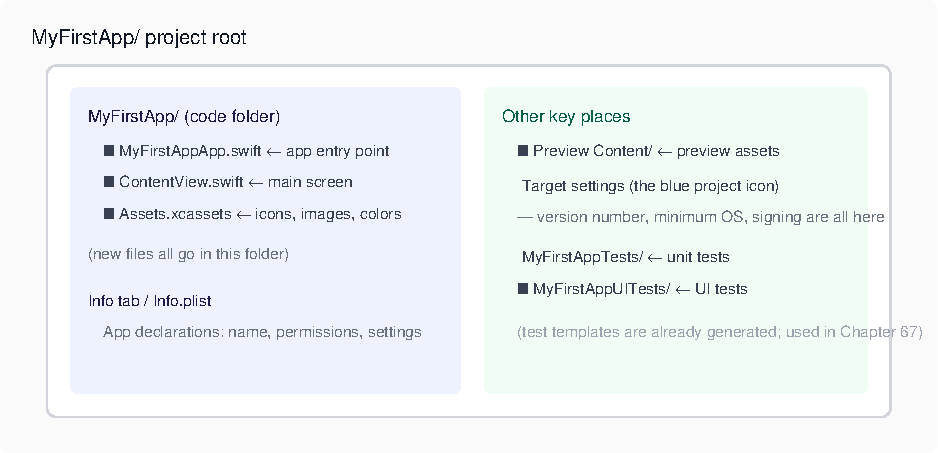
\includegraphics[width=0.92\linewidth]{figures/fig-di-liu-shi-zhang-1}
\\[2pt]\small Figure 2: The Xcode project structure every beginner must know
\end{center}

\begin{itemize}
  \item MyFirstAppApp.swift: the program's entry point. In SwiftUI it's only a few lines—"launch, then show the main screen";
  \item ContentView.swift: the main screen view—everything you're looking at right now lives here;
  \item Assets.xcassets: the resource warehouse—icons, images, and colors all go here;
  \item Target settings: click the blue project icon on the left to get in. The version number, the minimum iOS version, and signing are all in there. The app's display name and icon are configured here too.
\end{itemize}

\booksection{Testing on a Real Device: Install the App on Your iPhone}

\booksection{Xcode Efficiency Tricks: Five “Shortcut Power-Ups” for Beginners}

Get fluent with these and you'll look “very professional”:

\begin{center}
\begin{tabularx}{\linewidth}{|X|X|X|}
\hline
\textbf{Action} & \textbf{Shortcut} & \textbf{What it does} \tabularnewline
\hline
Run & CmdR & Build and run \tabularnewline
Open/toggle the canvas preview & OptionCmd & The what-you-see-is-what-you-get switch \tabularnewline
Re-indent & CtrlI & Automatically tidy up the indentation of the selected code \tabularnewline
Quick Open & CmdO & Type a file name and it opens instantly (the most used!) \tabularnewline
Comment/uncomment & Cmd/ & Switch code on and off while debugging \tabularnewline
\hline
\end{tabularx}
\end{center}

\begin{center}\small\color{gray}High-frequency Xcode shortcuts (the beginner's five)\end{center}

Two more hidden perks: multiple simulators at once (run an iPhone and an iPad side by side to compare layouts) and the snippet library (drag a few lines of frequently used code into the Snippets panel on the right, then insert them with one click next time)—use these efficiency tools early, and the fluency will follow naturally.

\booksection{Testing on a Real Device: Install the App on Your iPhone}

The simulator is nice, but a real device is the destination. You can test on a real device even with a free Apple ID:

\begin{enumerate}
  \item Connect your iPhone with a cable (or debug wirelessly over the same Wi-Fi);
  \item Pick your phone from the device list at the top of Xcode; the first time, you'll be asked to sign in with your Apple ID and signing gets configured automatically;
  \item On the iPhone, go to [Settings] > [General] > [VPN \& Device Management] and trust your developer certificate;
  \item Click >, and the app lands on your real device.
\end{enumerate}

\begin{tcbwarn}{Note: The Free Account's "Seven-Day Limit"}
An app signed with a free Apple ID stops working after 7 days (just run it again to renew). This is Apple's anti-abuse mechanism, and it's completely fine for the learning stage; a paid developer account (\$99/year) has no such limit—Chapter 67 has the details.

\end{tcbwarn}

\booksection{Try It Yourself + First Aid for Common Errors}

\booksection{Try It Yourself + First Aid for Common Errors}

Open ContentView.swift, change the text inside Text(“Hello, world!”) to your name, and press CmdR to run again—a few seconds later, your name shows up on the simulator. Congratulations: you've completed your first full “edit code build install run” loop.

\begin{center}
\begin{tabularx}{\linewidth}{|X|X|X|}
\hline
\textbf{Symptom} & \textbf{Common cause} & \textbf{The fix} \tabularnewline
\hline
Signing error & No Team selected, or an expired certificate & In Target > Signing, check your account; with a free account, just run again \tabularnewline
Simulator shows a black screen / won't open & Corrupted simulator image & Menu: Device > Erase All Content; or delete the simulator and add it again \tabularnewline
Xcode downloads slowly / won't install & App Store network hiccup & Try a different time of day; or download the .xip offline installer from the Apple developer website \tabularnewline
\hline
\end{tabularx}
\end{center}

\begin{center}\small\color{gray}First-aid table for beginner environment errors\end{center}

\begin{tcbpractice}{Hands-on: Finish Your "Developer Initiation" Checklist}
1) Install Xcode and get the simulator running; 2) run your app on a real device once and take a screenshot to mark the occasion; 3) change the Hello text to your name; 4) go to the Target settings and change the app's display name to “My First App.” Once these four steps are done, you're officially someone with a creation of your own.

\end{tcbpractice}

\begin{tcbsummary}{Chapter summary}
\begin{itemize}
  \item Hard requirements: a Mac + Xcode; no Mac yet? Learn the language first with Swift Playgrounds on the iPad
  \item Install Xcode from the App Store; new versions demand new systems, so don't put off updates
  \item The five essentials of a new project: name, Team, organization identifier, SwiftUI, Swift
  \item The project mantra: all your code lives in the MyFirstApp/ folder; Target settings manage the version and signing
  \item Real-device testing with a free Apple ID has a 7-day signing limit; a paid account has no such limit
  \item The developer's daily routine = edit code CmdR see the result, over and over
\end{itemize}

\end{tcbsummary}
